\section{Algebraic Point Set Surfaces}

The Algebraic Point Set Surfaces \cite{Guennebaud07} falls into the category of so-called point set surfaces, where the approximate signed distance function to the inferred surface can be evaluated at any query point, on the fly during iso-contouring: \\
\ccc{CGAL::APSS_reconstruction_function<GeomTraits>}  \\

% Insert image APSS.jpg/eps
\begin{center}
    \label{Surface_reconstruction_points_3-fig-APSS}
    % Image
    \begin{ccTexOnly}
        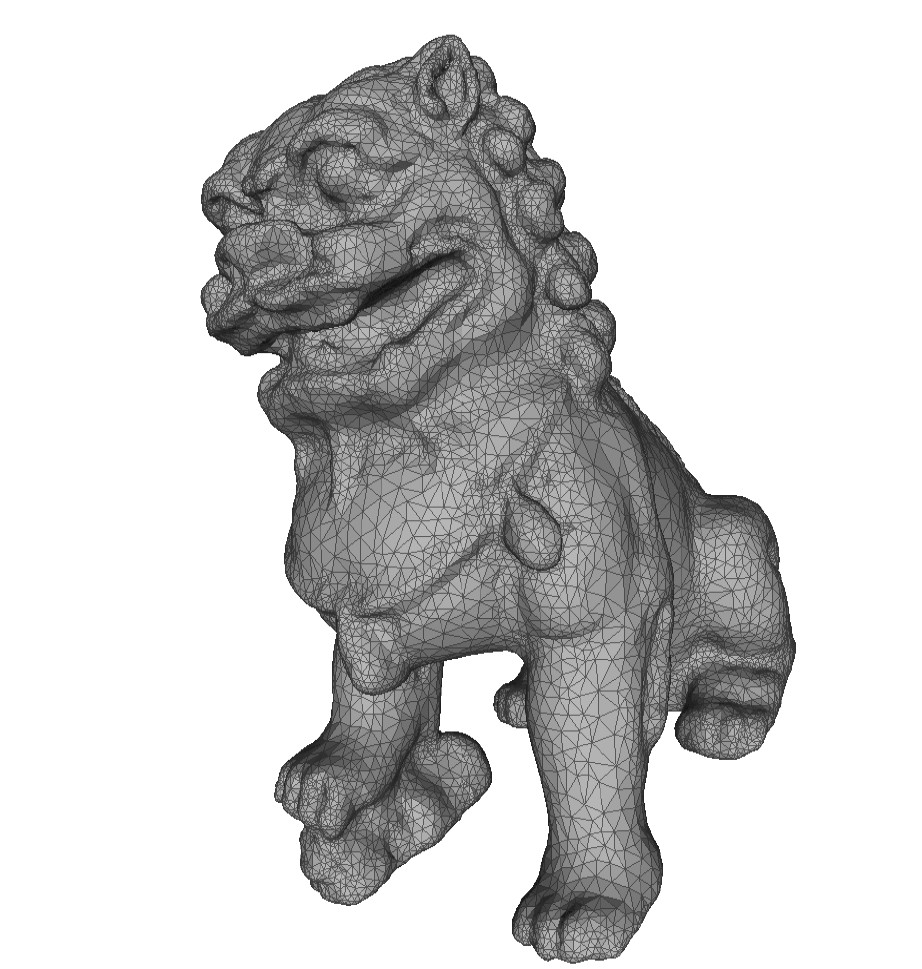
\includegraphics[width=0.5\textwidth]{Surface_reconstruction_points_3/APSS} % omit .eps suffix
    \end{ccTexOnly}
    \begin{ccHtmlOnly}
        <img width="50%" border=0 src="./APSS.jpg"><P>
    \end{ccHtmlOnly}
    % Title
    \begin{figure}[h]
        \caption{APSS surface reconstruction from 10K
                 points sampled with a Minolta laser scanner.}
        % later: add computed function
    \end{figure}
\end{center}


\emph{more to come here about interface and example}

%\subsection{Interface}
%\subsection{Example}

